\documentclass[11pt,a4paper]{amsart}
\usepackage[T1]{fontenc}
\usepackage{lmodern}
\usepackage{amsmath,amssymb,amsthm,booktabs}
\usepackage[margin=30mm]{geometry}
\usepackage{pgfplots}
\pgfplotsset{compat=1.17}
\usepgfplotslibrary{groupplots}
\definecolor{boundblue}{HTML}{0072B2}
\definecolor{pathorange}{HTML}{D55E00}
\usepackage[hidelinks]{hyperref}
\raggedbottom
\renewcommand{\topfraction}{.9}\renewcommand{\textfraction}{.08}\renewcommand{\floatpagefraction}{.8}
\newtheorem{theorem}{Theorem}[section]
\newtheorem{lemma}[theorem]{Lemma}
\newtheorem{proposition}[theorem]{Proposition}
\theoremstyle{definition}
\newtheorem{definition}[theorem]{Definition}
\theoremstyle{remark}
\newtheorem{remark}[theorem]{Remark}
\newcommand{\N}{\mathbb N}
\title[Finite-depth Collatz certification]{Finite-depth Collatz certification through sharp first-crossing envelopes}
\date{October 9, 2026}
\subjclass[2020]{Primary 11B83; Secondary 37P99}
\keywords{Collatz iteration, coefficient stopping time, mechanical word, finite certificate}
\begin{document}
\begin{abstract}
We study the gap between coefficient contraction and actual descent in the
shortcut Collatz map. The first-contraction constraint determines a unique
rightmost feasible parity word, whose affine offset is maximal. This sharp
envelope reduces certification at depth $K$ to an explicit finite set of
potential exceptions, without enumerating $2^K$ residue classes. At
$K=1024$, exact arithmetic gives the exception bound $72058$. Independent
verification of this finite range proves that every integer $n>1$ with
coefficient stopping time at most 1024 has equal actual stopping time.
An independent first-passage recurrence counts the unclassified residue
mass, approximately $1.1537401\times10^{-19}$ at this depth.
We also derive the asymptotic normalized envelope $1/(6\log2)$ and show why
neither a fixed depth nor a fixed envelope scan limit proves universal
descent. This is a self-contained computational study of established
parity-vector methods; no priority claim or resolution of the general
conjecture is made.
\end{abstract}
\maketitle

\section{Question, context, and principal conclusion}
Let
\begin{equation}\label{eq:T}
T(n)=\begin{cases}n/2,&n\equiv0\pmod2,\\(3n+1)/2,&n\equiv1\pmod2,\end{cases}
\end{equation}
on the positive integers. Write $q_j(n)$ for the number of odd terms among
the first $j$ iterates, including $n$ and excluding $T^j(n)$, and define
\[
C_j(n)=\frac{3^{q_j(n)}}{2^j},\qquad
\tau(n)=\min\{j\ge1:C_j(n)<1\},\quad
\sigma(n)=\min\{j\ge1:T^j(n)<n\}.
\]
An empty minimum is $\infty$. All statements about equality of these
stopping times below exclude $n=1$, for which $\tau(1)=2$ and
$\sigma(1)=\infty$.

The conjecture that $\sigma(n)=\tau(n)$ for all $n\ge2$ is usually called
the coefficient stopping time conjecture, following Terras~\cite{Terras}.
Rozier and Terracol~\cite{RT} discuss its relation to finite trajectories
with coefficient below one but endpoint at least the starting value.
Their example $7,11,17,26,13,20,10,5,8$ illustrates why contraction at an
arbitrary later time is insufficient: the coefficient at step 8 is
$243/256<1$, yet the endpoint is 8. This does not violate the conjecture,
because descent already occurred at step 7.

The present question is computational and conditional: can the equality
be certified at a large \emph{first-contraction depth}, uniformly over
all starting integers, without constructing the entire parity tree?
The principal finite conclusion is the following.

\begin{theorem}[Exact finite-depth certificate]\label{thm:main}
For every positive integer $n>1$,
\[
\tau(n)\le1024\quad\Longrightarrow\quad\sigma(n)=\tau(n).
\]
There is no size restriction on $n$. The implication makes no assertion
when $\tau(n)>1024$ or $\tau(n)=\infty$.
\end{theorem}

The proof combines an elementary sharp envelope, a finite reduction, and
the accompanying exact certificate checks. A complete derivation follows;
the numerical part is isolated in Section~\ref{sec:results}.
Parity classes and offset comparisons are established tools, and the
literature reports much larger computational investigations than the
small scan used here. The purpose is a transparent, independently
replayable reduction, not a new verification record or a claim that the
general stopping-time conjecture has become tractable.

\section{Affine identities and first-crossing constraints}
For a binary word $w=(\varepsilon_0,\ldots,\varepsilon_{k-1})$, let
$a_j=\sum_{i<j}\varepsilon_i$. On the integers realizing this parity word,
\begin{equation}\label{eq:affine}
T^j(n)=\frac{3^{a_j}n+B_j}{2^j},\qquad B_0=0,
\end{equation}
where
\begin{equation}\label{eq:B}
B_{j+1}=\begin{cases}B_j,&\varepsilon_j=0,\\
3B_j+2^j,&\varepsilon_j=1.\end{cases}
\end{equation}
Each word is realized by exactly one residue class modulo $2^k$.
To see this, suppose a word of length $j$ has residue $r$.
Its two lifts $r$ and $r+2^j$ have $j$th iterates differing by the odd
integer $3^{a_j}$, so they realize opposite next parities. Induction
proves both the residue assertion and~\eqref{eq:affine}.
All offsets are nonnegative. Hence actual descent requires coefficient
contraction, and
\begin{equation}\label{eq:order}
\sigma(n)\ge\tau(n).
\end{equation}

Set $\alpha=\log_3 2$ and define the exact barrier
\begin{equation}\label{eq:h}
h_j=\min\{a\ge0:3^a\ge2^j\},\qquad h_0=0.
\end{equation}
For $j>0$, $h_j=\lceil\alpha j\rceil$; equality of positive powers of 2
and 3 is impossible. Since $0<\alpha<1$, successive barrier increments
are either zero or one. In implementation,~\eqref{eq:h} is evaluated by
integer comparisons, never by rounding logarithms.

\begin{lemma}\label{lem:cross}
If a word first contracts at depth $k$, its last bit is zero and its total
odd count is $q=h_{k-1}$. Such a word exists exactly when
\begin{equation}\label{eq:feasible}
2^{k-1}\le3^{h_{k-1}}<2^k.
\end{equation}
All its proper prefix counts obey $a_j\ge h_j$ for $j<k$.
\end{lemma}
\begin{proof}
An odd step multiplies the coefficient by $3/2$, and therefore cannot be
the first contraction. At the preceding depth the coefficient is at
least one, so $2^{k-1}\le3^q<2^k$. This interval contains at most one
power of 3 and, if it contains one, its exponent is $h_{k-1}$.
Noncontraction of each earlier prefix gives the barrier condition.
Conversely, the word whose prefix counts are $h_j$ for $j<k$, followed
by a zero bit, realizes first contraction whenever~\eqref{eq:feasible}
holds. All these counts are achievable because barrier increments are
binary.
\end{proof}

\section{A sharp constrained offset envelope}
For every feasible $k$, let $w_k^*$ have proper prefix counts exactly
$h_j$ and final bit zero. Denote its offset by $M_k$. This construction
postpones each odd step as far as the prefix barriers permit.

\begin{theorem}[Sharp first-crossing envelope]\label{thm:envelope}
Among all words first contracting at a feasible depth $k$, $w_k^*$ is the
unique word with maximal offset. If $q=h_{k-1}$ and the odd positions of
a word are $i_1<\cdots<i_q$, then
\begin{equation}\label{eq:positions}
B_k=\sum_{\ell=1}^q3^{q-\ell}2^{i_\ell},\qquad
i_\ell\le i_\ell^*:=\lfloor(\ell-1)\log_2 3\rfloor.
\end{equation}
Thus $B_k\le M_k$, with equality only for $w_k^*$.
For $q=0$, the sole word is the even one-step word and $M_1=0$.
\end{theorem}
\begin{proof}
Each odd step inserts $2^{i_\ell}$ in~\eqref{eq:B}; each later odd step
multiplies that contribution by 3. Summing gives the first identity.
The barrier first reaches $\ell$ at
\[
j_\ell=\min\{j:h_j\ge\ell\}
=\lfloor(\ell-1)\log_2 3\rfloor+1.
\]
Every feasible word must already have $\ell$ odd positions among its
first $j_\ell$ bits. Therefore $i_\ell\le j_\ell-1=i_\ell^*$.
The proposed word attains all these upper bounds simultaneously.
Every summand in~\eqref{eq:positions} strictly increases with its
position, proving maximality and uniqueness. This argument does not
require a sequence of swaps to remain feasible at every intermediate word.
\end{proof}


\subsection*{A complete small example}
At $k=8$, the barrier values $(h_0,\ldots,h_8)$ are
$(0,1,2,2,3,4,4,5,6)$. The extremal word is $11011010$, with
odd positions $0,1,3,4,6$, so
\[
M_8=3^4+3^3\,2+3^2\,2^3+3\,2^4+2^6=319.
\]
The word $11111000$ is also a first-crossing word, but its earlier odd
positions give offset $211$. Both have $q=5$ and coefficient
$243/256$ at depth 8. Figure~\ref{fig:barrier} exhibits the prefix
constraint responsible for their different offsets.

\begin{figure}[!ht]
\centering
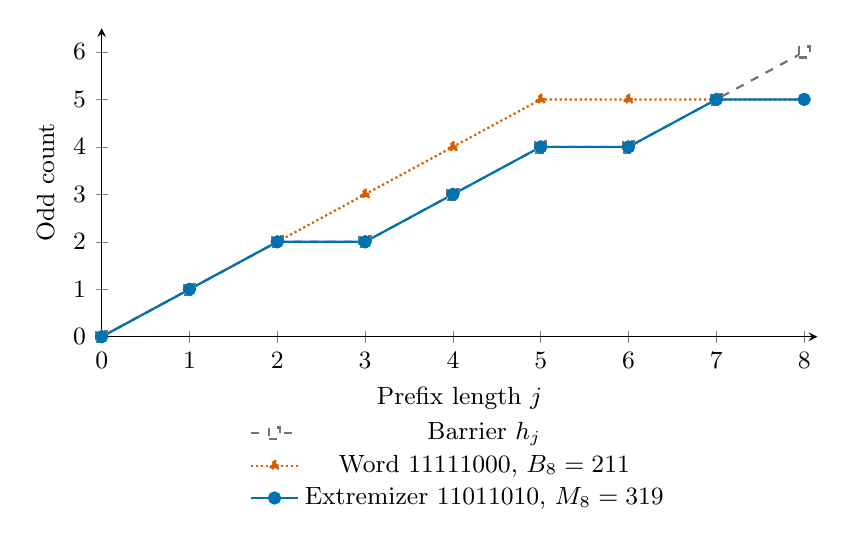
\begin{tikzpicture}
\begin{axis}[width=.88\linewidth,height=5.5cm,xmin=0,xmax=8.15,ymin=0,ymax=6.5,
 xlabel={Prefix length $j$},ylabel={Odd count},xtick={0,1,2,3,4,5,6,7,8},ytick={0,1,2,3,4,5,6},
 tick label style={font=\small},label style={font=\small},
 legend style={font=\small,at={(.5,-.24)},anchor=north,draw=none,fill=white},
 axis lines=left]
\addplot[black!55,dashed,mark=square*,mark options={fill=white},thick] coordinates {(0,0)(1,1)(2,2)(3,2)(4,3)(5,4)(6,4)(7,5)(8,6)};
\addlegendentry{Barrier $h_j$}
\addplot[pathorange,densely dotted,mark=triangle*,thick] coordinates {(0,0)(1,1)(2,2)(3,3)(4,4)(5,5)(6,5)(7,5)(8,5)};
\addlegendentry{Word $11111000$, $B_8=211$}
\addplot[boundblue,mark=*,thick] coordinates {(0,0)(1,1)(2,2)(3,2)(4,3)(5,4)(6,4)(7,5)(8,5)};
\addlegendentry{Extremizer $11011010$, $M_8=319$}
\end{axis}
\end{tikzpicture}
\caption{First crossing at depth 8. Counts must stay at or above the barrier at every proper prefix and fall below it at the last step. Lines connect integer-depth observations only. Delaying odd positions within these constraints maximizes the affine offset; an unconstrained late-odd word need not obey the barriers.}
\label{fig:barrier}
\end{figure}

An exhaustive check of the 256 residues modulo $256$ gives seven words
with first crossing at depth 8 and confirms that the largest offset is
319. The two illustrated words correspond respectively to residues 123
and 95. In particular, a positive integer realizing the extremal word
is at least 123, whereas its failure bound is
$\lfloor319/(256-243)\rfloor=24$. Thus that class contains no failure.
This example also shows why the uniform envelope is a sufficient bound:
it discards the residue restriction, which may sharpen individual cases.

The unconstrained maximum for fixed length $k$ and odd count $q$ instead
puts all odd bits at the end. It equals
\begin{equation}\label{eq:general}
U_{k,q}=2^{k-q}(3^q-2^q).
\end{equation}
Indeed, the largest possible odd positions are $k-q,\ldots,k-1$;
substitution in~\eqref{eq:positions} gives~\eqref{eq:general}.
That word normally contracts long before its last step, so the bound
throws away the crucial first-crossing information. At $k=485$, $q=306$,
its ratio to $M_k$ is approximately $1.03971\times10^{52}$.
This is a comparison of mathematical bounds, not a measured runtime
speedup against all existing Collatz algorithms.

\begin{theorem}[Finite reduction]\label{thm:reduction}
For an integer $K\ge1$, define
\begin{equation}\label{eq:H}
H_K=\max_{\substack{k\le K\\k\text{ feasible}}}
\left\lfloor\frac{M_k}{2^k-3^{h_{k-1}}}\right\rfloor.
\end{equation}
If every integer $2\le n\le H_K$ with $\tau(n)\le K$ satisfies
$T^{\tau(n)}(n)<n$, then every $n>1$ with $\tau(n)\le K$ satisfies
$\sigma(n)=\tau(n)$.
\end{theorem}
\begin{proof}
Let $\tau(n)=k\le K$ and put $A=3^{h_{k-1}}$, $D=2^k$.
By~\eqref{eq:affine} and Theorem~\ref{thm:envelope},
\[
T^k(n)\ge n\quad\Longrightarrow\quad
(D-A)n\le B_k\le M_k\quad\Longrightarrow\quad n\le H_K.
\]
The hypothesized finite check excludes such a failure for $n>1$.
Therefore descent occurs at time $k$. Equation~\eqref{eq:order} rules
out an earlier descent and yields equality of the stopping times.
The weak inequality at the failure boundary is essential: the floor in
\eqref{eq:H} must include equality, not discard it as a strict comparison.
\end{proof}

\section{Compressed counting and independent checks}
For counting purposes only, write $s_{j,a}$ for the number of length-$j$
words having $a$ odd bits and no contracted prefix. Initialize
$s_{0,0}=1$. Each state contributes to odd counts $a$ and $a+1$ at the
next depth; retain the contribution precisely if $3^a\ge2^{j+1}$ or
$3^{a+1}\ge2^{j+1}$, respectively. Let $F_j$ count words whose first
contraction occurs at $j$, and $R_K=\sum_a s_{K,a}$. The disjoint
first-passage decomposition gives
\begin{equation}\label{eq:mass}
R_K=2^K-\sum_{j=1}^K F_j2^{K-j},\qquad
\rho_K=\frac{R_K}{2^K}.
\end{equation}
By the parity-residue bijection, $\rho_K$ is the natural density of
$\{n:\tau(n)>K\}$. It is not a sampled frequency or a probability of
divergence. After finite-depth equality is certified, it is also the
density of $\{n:\sigma(n)>K\}$; deleting the exceptional point 1 does
not change a natural density.

The production code computes barriers, extremal offsets, and forward
counts using integer arithmetic. There are $O(K^2)$ counting-state
updates, instead of enumerating all $2^K$ words. This counts arithmetic
operations; integers have increasing bit length, so it is not an
$O(K^2)$ bit-complexity claim. Explicit certificate rows retain the
large integers needed to replay the thresholds.

The checker uses two different recurrences. For extrema, it keeps the
maximum offset in each surviving state $(j,a)$, applies the affine update
to both next bits, and records maxima at first crossings. This max-plus
calculation does not use the rightmost-word formula. For counts, it uses
binomial renewal instead of the forward state recursion. At a feasible
depth $k$, with $q_k=h_{k-1}$,
\begin{equation}\label{eq:renewal}
F_k=\binom{k-1}{q_k}
-\sum_{\substack{j<k\\j\text{ feasible}}}
F_j\binom{k-1-j}{q_k-q_j},
\end{equation}
where a binomial coefficient outside its usual range is zero. The first
term counts all prefixes of length $k-1$ having $q_k$ odd bits. The sum
removes those with an earlier first crossing; their remaining bits are
arbitrary. Appending a zero produces the crossing at $k$.
For an infeasible $k$, $F_k=0$.

Finite trajectories are checked separately: iterate each integer through
its first coefficient contraction and compare the actual endpoint with
the initial value. Reaching the cap without coefficient contraction is
reported outside the theorem, not as a counterexample or a success.
The checker also verifies complete depth and domain coverage and rejects
six damaged certificates: wrong offset, wrong threshold, missing crossing
depth, wrong density, shortened scan domain, and altered scan histogram.
The verifier uses explicit exceptions rather than assertion-dependent
acceptance. An author-independent review additionally rederived the
extremal bound, checked all first-crossing words through depth 18, and
recomputed the depth-1024 extrema and finite trajectories.

\section{Exact results}\label{sec:results}
\begin{table}[ht]
\centering
\caption{Finite-depth envelopes and exact-count residue densities.
The densities are displayed approximately; the certificate retains exact
integer numerators and denominators.}
\label{tab:main}
\begin{tabular}{rrrr}
\toprule
$K$&$H_K$&Depth attaining $H_K$&$\rho_K$\\
\midrule
16&24&8&$3.2257080\times10^{-2}$\\
32&108&27&$9.6269611\times10^{-3}$\\
64&281&46&$1.4930654\times10^{-3}$\\
128&867&65&$6.9777999\times10^{-5}$\\
256&4862&233&$3.2760221\times10^{-7}$\\
512&72058&485&$1.6152967\times10^{-11}$\\
1024&72058&485&$1.1537401\times10^{-19}$\\
\bottomrule
\end{tabular}
\end{table}


Figure~\ref{fig:tradeoff} separates two effects of increasing depth:
the remaining residue density falls, while the sufficient scan bound
jumps when a new extremal depth is encountered. Density and scan size
measure different objects and are not combined into a single accuracy score.
\begin{figure}[!ht]
\centering
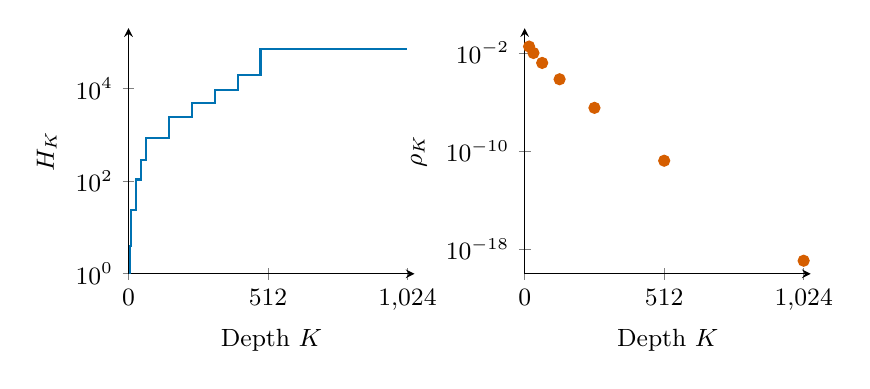
\begin{tikzpicture}
\begin{groupplot}[group style={group size=2 by 1,horizontal sep=1.4cm},width=.43\linewidth,height=4.7cm]
\nextgroupplot[xmin=0,xmax=1050,ymode=log,
 ymin=1,ymax=200000,xlabel={Depth $K$},ylabel={$H_K$},
 xtick={0,512,1024},ytick={1,100,10000},axis lines=left,
 tick label style={font=\small},label style={font=\small}]
\addplot[boundblue,thick,const plot] coordinates {(2,1)(5,4)(8,24)(27,108)(46,281)(65,867)(149,2419)(233,4862)(317,9266)(401,19584)(485,72058)(1024,72058)};


\nextgroupplot[xmin=0,xmax=1050,ymode=log,
 ymin=1e-20,ymax=1,xlabel={Depth $K$},ylabel={$\rho_K$},
 xtick={0,512,1024},ytick={1e-2,1e-10,1e-18},axis lines=left,
 tick label style={font=\small},label style={font=\small}]
\addplot[pathorange,only marks,mark=*,mark size=2pt] coordinates {(16,0.032257080078125)(32,0.0096269610803574324)(64,0.0014930653834529545)(128,6.9777998782994224e-05)(256,3.2760221243761753e-07)(512,1.6152966911049405e-11)(1024,1.1537400846119692e-19)};

\end{groupplot}
\end{tikzpicture}
\caption{Two exact-count summaries from the depth-1024 certificate, shown on separate logarithmic scales. Left: the sufficient exception bound is a step function (the zero value at $K=1$ is omitted on the log scale). Right: unclassified natural density at the seven tabulated checkpoints; no interpolation is implied. The small final density is positive and does not establish universal descent.}
\label{fig:tradeoff}
\end{figure}

At depth 1024 there are 647 feasible first-crossing lengths. The largest
exception floor occurs at $(k,q)=(485,306)$ and is 72058.
For that pair, the unconstrained offset bound~\eqref{eq:general} would
give a scan limit of approximately $7.49195\times10^{56}$.
The reduction to 72058 is the practical role of the prefix constraint.
The finite scan examines all 72057 integers from 2 through 72058.
There are no endpoint failures and no capped trajectories.
The largest coefficient stopping time in this scan is 135, attained only
at 35655; this is a statistic of the finite scan, not an upper bound for
all integers in Theorem~\ref{thm:main}.

\begin{proof}[Proof of Theorem~\ref{thm:main}]
The exact certificate gives $H_{1024}=72058$. The independent max-plus
recurrence confirms every extremal offset and every threshold at the 647
feasible depths. Direct finite replay checks the hypothesis of
Theorem~\ref{thm:reduction} on every required initial integer.
That theorem gives the asserted implication uniformly over all $n>1$.
The certificate object, checking program, and completed run are part of
the finite computational evidence, not a replacement for the preceding
mathematical reduction.
\end{proof}

The generating calculation took about 0.065 seconds, including the
finite scan and 387646 forward state updates. The independently coded
checker took about 0.639 seconds, including max-plus extrema, binomial
renewal, finite replay, and negative controls. These are observations
on the recorded Python 3.12 environment, not universal benchmark timings.
They exclude derivation, literature reading, review, and manuscript work.
Fast arithmetic does not by itself indicate a deep mathematical result.

The earlier depth-16 explicit tree is retained as a separate baseline.
Its 791 leaf words and 2114 unresolved residues agree exactly with the
compressed count. The new result changes the scope from an explicit
small tree and an unrelated finite scan to a uniform first-depth theorem;
it does not merely enlarge the initial integer range.

\section{Envelope asymptotics and limits of continuation}
The extremizer also describes how the sufficient scan bound behaves.
Set $\beta=\log_2 3$, and for $q\ge1$ let
$k_q=\lfloor q\beta\rfloor+1$. These are exactly the feasible crossing
lengths other than $k=1$. Put $\delta_q=k_q-q\beta\in(0,1)$.

\begin{proposition}\label{prop:asymptotic}
For $q\ge1$,
\begin{equation}\label{eq:normalized}
\frac{M_{k_q}}{3^q}
=\frac13\sum_{\ell=0}^{q-1}2^{-\{\ell\beta\}},\qquad
\frac{M_{k_q}}{q3^q}\longrightarrow\frac1{6\log2}.
\end{equation}
In particular,
\begin{equation}\label{eq:growth}
\left\lfloor\frac{M_{k_q}}{2^{k_q}-3^q}\right\rfloor
>\frac q6-1.
\end{equation}
Thus the sufficient scan limit $H_K$ is unbounded as $K\to\infty$.
This does not assert that any genuine exception exists.
\end{proposition}
\begin{proof}
Divide~\eqref{eq:positions} at the maximizing positions by $3^q$.
Since $2^\beta=3$, its $\ell$th summand becomes
$2^{-\{(\ell-1)\beta\}}/3$, proving the identity.
The number $\beta$ is irrational: a rational value would give equality
of nontrivial integer powers of 2 and 3.
For any nonzero integer $m$, the average of
$\exp(2\pi i m\ell\beta)$ tends to zero by the finite geometric-series
formula. Weyl's criterion therefore gives uniform distribution of
$\{\ell\beta\}$; see~\cite{TaoNotes}, Proposition 1 and Exercise 5.
Applying it to the bounded Riemann-integrable function $2^{-x}$ on
$[0,1)$ gives
\[
\frac1{3q}\sum_{\ell<q}2^{-\{\ell\beta\}}
\longrightarrow\frac13\int_0^1 2^{-x}\,dx=\frac1{6\log2}.
\]
The single endpoint discontinuity on the circle is harmless: continuous
upper and lower approximations can differ only on an interval of
arbitrarily small length, whose asymptotic frequency equals its length.
Every summand in the normalized sum is greater than $1/6$, and
$2^{\delta_q}-1<1$. Consequently
\[
\frac{M_{k_q}}{2^{k_q}-3^q}
=\frac{M_{k_q}/3^q}{2^{\delta_q}-1}>\frac q6.
\]
Taking the floor proves~\eqref{eq:growth} and unboundedness.
\end{proof}

For illustration, $M_{k_q}/(q3^q)$ equals approximately 0.249815 at
$q=17$, 0.240844 at $q=306$, and 0.240668 at $q=646$; the limit is
approximately 0.240449. These finite values illustrate the proved limit,
but neither establish a finite error rate nor prove monotonic convergence.
The denominator $2^{\delta_q}-1$ explains large jumps of the envelope
when a power of 3 is close to a power of 2 from below.

\begin{proposition}[No fixed-horizon coverage]\label{prop:obstruction}
For every $K\ge1$, there is an $n>1$ with $\tau(n)>K$ and $\sigma(n)>K$.
\end{proposition}
\begin{proof}
For $K\ge2$, take $n=2^K-1$. Direct induction gives
\[
T^j(n)=3^j2^{K-j}-1\qquad(0\le j\le K).
\]
The terms before the last are odd, and each term with $j\ge1$ is larger
than $n$. The coefficient is $(3/2)^j>1$. For $K=1$, take $n=3$.
\end{proof}

Thus the very small density in Table~\ref{tab:main} cannot be rounded to
zero or read as universal convergence. Nor can the finite theorem be
iterated without an argument controlling the unclassified starting
values. Proposition~\ref{prop:asymptotic} identifies another limitation:
this particular uniform envelope cannot certify all crossing depths by
one fixed finite scan. It does not prove that other methods fail, and it
does not show that the coefficient stopping time conjecture is false.

\section{Research status and reproducibility}
The study has three different evidence types: elementary proofs of the
envelope and reduction, exact finite checks for the depth-1024 instance,
and a qualitative asymptotic deduction from classical equidistribution.
The recorded decimals are presentation values; all certificate decisions
use integers. No random sampling, learned model, or fitted threshold is
used. No proof assistant verifies the Python runtime or the entire paper.

From the revision directory, the standard-library entry points are
\begin{quote}\small\ttfamily
python code/certify.py\\
python code/verify.py
\end{quote}
The certificate records every feasible depth, offset, exact threshold,
density fraction, and finite scan summary. Separate review artifacts
contain the author-independent calculations. Version hashes and the
actual environment accompany the manuscript; generating a new run should
be done in a copy if the sealed research record is to remain unchanged.

The main unresolved issue is structural. The all-integer conjecture needs
control beyond every fixed first-crossing depth, or a genuinely different
argument for the residual cases. Enlarging 1024 without such an argument
would produce another finite certificate, not resolve that issue.
The present continuation therefore stops after the validated reduction
and its limitations. Originality of the constrained envelope as a
standalone result has not been established; the local study is presented
as a verified synthesis and computational note rather than a new general
Collatz theorem.

\begin{thebibliography}{9}
\bibitem{RT} O. Rozier and C. Terracol, \emph{Paradoxical behavior in
Collatz sequences}, Discrete Math. \textbf{349} (2026), Article 115167.
\href{https://arxiv.org/abs/2502.00948v5}{arXiv:2502.00948v5}.
\bibitem{TaoNotes} T. Tao, \emph{254B, Notes 1: Equidistribution of
polynomial sequences in tori}, lecture notes, March 28, 2010,
\href{https://terrytao.wordpress.com/2010/03/28/254b-notes-1-equidistribution-of-polynomial-sequences-in-torii/}{author's online notes}.
\bibitem{Terras} R. Terras, \emph{A stopping time problem on the positive
integers}, Acta Arith. \textbf{30} (1976), 241--252.
\href{https://doi.org/10.4064/aa-30-3-241-252}{doi:10.4064/aa-30-3-241-252}.
\end{thebibliography}
\end{document}
